%!TEX root = ../main.tex
%=========================================================

\section{Introduction}

Ethereum~\cite{buterin2013ethereum}  is the largest permission-less (\ie open membership), open-source blockchains supporting Turing-complete scripting via smart contracts. 
In addition to running its own blockchain platform, Ethereum is home to third-party decentralized applications and platforms that run alternative cryptocurrencies (Pirl, Musicoin) and host various services such as content delivery (Swarm) or messaging (Whisper).
A vast majority of these applications require dedicated \emph{sub-networks}, each consisting of only the peers participating in a particular application. A \emph{sub-network} enables the exchange of application-specific data, such as transactions and blocks, only between the interested peers. In 2018, the Ethereum P2P network nodes operated a total of 4,076 different applications (\Cref{fig:ecosystem}), and this number is expected to grow in the future~\cite{kim2018measuring} .

\begin{figure}
    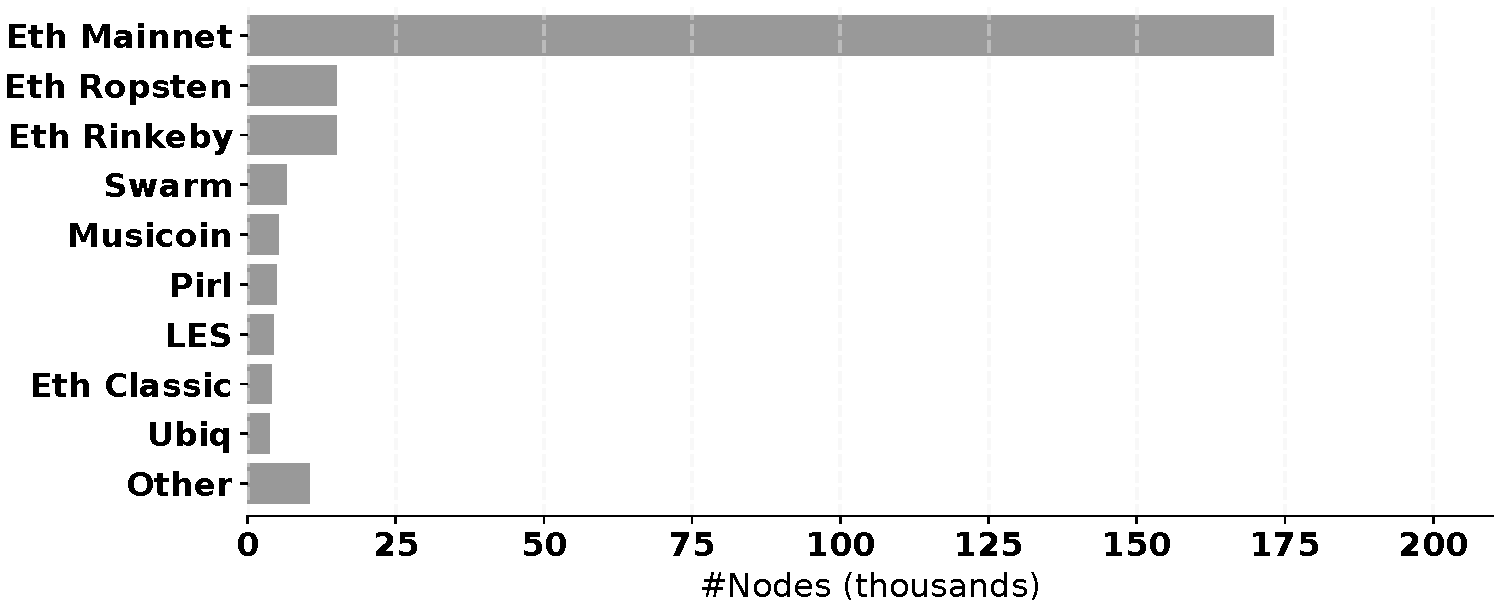
\includegraphics[width=1\linewidth]{img/ecosystem}
    \caption{Sub-networks in the Ethereum ecosystem.}
    \label{fig:ecosystem}
\end{figure}

Before a sub-network can be formed, its peers must first discover each other. The process of finding application-specific peers is crucial for the security of the entire system. Operations of even largest networks can be effectively disrupted when its nodes cannot find each other. Worse even, a node using an unreliable service discovery protocol may be fed a list of malicious nodes and become completely eclipsed from the network. In the context of blockchains and cryptocurrency, service discovery eclipse attacks can lead to double-spent attacks, stubborn mining and hinder security of assets currently worth billions of USD. 

\para{State-of-the-art} Currently, Ethereum provides Discv4 - a decentralized, general purpose \textit{service discovery protocol} enabling any node to discover \textit{a random sample} of peers running a desired application. A node first \textit{(i)} joins the (application-agnostic) Ethereum network, \textit{(ii)} discovers application-specific peers and \textit{(iii)} joins a sub-network by connecting to the discovered peers. The protocol is based on Kademlia~\cite{maymounkov2002kademlia} – a well-established Distributed Hash Table (DHT) implementation. Discv4 uses a simple, brute-force discovery mechanism involving random walks in the DHT containing peers from all ranges of applications. Each walk encounters random peers which are then supplied to the application. The application determines whether the supplied peers support the desired application through dedicated handshake messages. The process continues until a desired number of connection slots are filled. 

With the built-in randomness of the Kademlia peer selection mechanism, Discv4 is relatively secure against denial of service and eclipse attacks. Each nodes queries an unpredictable set of peers regardless of its application. As a result, an attacker cannot easily stop the process or strategically place its Sybil identities.
However, the overall process is highly inefficient, can take long time and generates significant message overhead. This is especially visible for unpopular applications with a small number of peers.  For instance, assuming an application with 10 nodes in a network of 5,000 nodes, a newcomer needs to perform an average 500 of handshakes to find a single peer. As more applications join the Ethereum network, the inefficiency of the brute-force discovery process becomes a bottleneck and prevents the growth of the entire ecosystem. 

%The randomness in the sampling of peers in both the DHT-level connections by Kademlia and application-level connections by Discv4 provides (a best-effort) Byzantine resilience in a permission-less network where financially-motivated attacks targeting individual applications are common. \er{I would not go as far as to write that it is Byzantine-resilient. It is a mitigation, but it has limits.} \er{is Kademlia used for something else than the random walk?}

%In addition to security, another major challenge facing service discovery is the \textit{scalability}: although random peer selection provides an acceptable-level of security against eclipsing attacks, the current discovery process is rather slow in finding peers for even moderately popular applications. \er{Does not strike me that discv4 is really subject to security problems, in the very worst case you could ask all peers in the network and would be guaranteed to get the $n$ ones you are looking for following topic $t$.} 
\dk{If large parts of the network are eclipsed, all nodes offering a certain topic/service might be unreachable. Eclipse attacks can prevent nodes from being able to ask all peers.}

\dk{Could provide a simple model showing this. I have done a basic calculation, which I will link in the PR.}
\dk{Waku v2\footnote{\url{https://wakunetwork.com}} is such an application. We discussed the shortcomings of random-walk discovery and are planning to implement more efficient means. You could list Waku as a motivation/example of an application that wants more efficient discovery means like the topic table this paper proposes.}

\para{Our Contribution} In this work, we propose \sysname - a new \textbf{service discovery layer} which enables secure,  efficient and robust discovery of application-specific peers in the Ethereum network.
Different from Discv4, \sysname allows nodes (\ie advertisers) to associate themselves with a set of \emph{topics} (\eg application IDs), and advertise the association (\ie an ad) in the network. 

The information is collectively stored by network participants (\ie registrars) without relying on a single trusted party at any point. Any node can then query the network for a topic to obtain a list of application-specific peers and directly connect to them without disturbing other members of the network. 

We build \sysname on top of the existing Kademlia DHT to propagate application-specific advertisements to randomly-sampled nodes to make deliberate attacks on the network costly to mount and persist. Our design encourages diversity of advertisements stored at each registrar making the system resistant to network dynamics and partitions. At the same time, \sysname provides efficient peer discovery operations terminating within a certain maximum number of steps (logarithmic in the network size) for all the topics regardless of their popularity. 

An open system allowing any node to place advertisement requires an admission protocol. Each registrar, having limited storage capacities, must decide which advertisement to accept and when should they expiry. This component is crucial for the system security and robustness in a highly dynamic environment. \sysname implements a lightweight admission mechanism to limit the resource usage on all the nodes, ensure fairness across topics, and prevent a vast range of malicious behaviours even in the presence of a powerful attacker.

\para{Contributions} We make the following contributions:
\begin{itemize}
    \item In \Cref{sec:placement}, we design a DHT-based data placement system that distributes service advertisement in the network. The protocol combines pseudo-random data placement for security with deterministic operations for efficiency. We present a lookup operation that finds a subset of advertisement placed in the system within a bounded amount of time. The procedure ensure the diversity of data sources and is resistant against manipulation by malicious registrars. 
    \item In \Cref{sec:registration} we design a lightweight admission protocol allowing advertisers to place ads after waiting for a specified amount of time. %\er{I would mention the problem and not only the solution here (make continuous registration of fake/malicious entries more complicated and limit their impact)}\mk{We've now added motivation for that in the paragraph just before the contributions} 
    \sysname guarantees that advertisers cannot place more advertisement at a specific registrar by deviating from the protocol %\er{is this completely true? I understood they could place more, but not many times more?}\mk{now it is. we ensure that with the lowe bound mechanism}
    and does not create any intermediary state at nodes holding the advertisements.
    \item In \Cref{sec:waitingTime}, we design a function that calculates a waiting time after which advertisement can be placed on nodes holding advertisements. The function limits the amount of resources used by each node, promotes ads diversity stored within nodes, and protects against a vast range of malicious behaviours. 
\end{itemize}

Our evaluations shows...


%Rather than each application building its own, dedicated peer discovery protocol where only the peers of individual applications participate, 


%The discovery process continues until an application-specific number of connections are successfully established with live peers. 
% \er{to discuss: ``service discovery'' could be understood as locating the single server in charge of a service--this term is often used in SOA. In the P2P world, I have seen the term ``membership management'' used as well to denote the discovery of a random set of peers from a group (seminal paper is SCAMP~\cite{ganesh2003peer}). We should preferably use the term used in the ETH community but we can give the precision in the RW section (I can do it).} % Onur: I think I addressed this now.





%An important feature of a large, general-purpose service discovery network is its ability to withstand security attacks: launching a successful attack against a protocol run by many applications' peers requires more resources than launching one against an application-specific discovery protocol with (at least initially) small number of participants. Security of the discovery protocol is especially crucial in the presence of financially-motivated attacks targeting cryptocurrency-based applications; a common one is a combination of \textit{eclipsing} and \textit{Sybil} attacks, whose purpose is to fill up a peer's connection slots to discovered peers with Sybils, which then collectively feed the peer incorrect information, \eg incorrect state of the application's blockchain, as part of a larger attack such as double-spending, stubborn mining, and so on. 

%For instance, a blockchain node that cannot find honest peers or is fully eclipsed by malicious peers might accept an incorrect state of the blockchain. These application-level attacks use as a precursor the more basic, targeted attacks such as eclipsing where an attacker aims to fill up a peer's application-level connections with its Sybils - afterwards, an application can be fed with any custom data as part of an attack such as double-spending, stubborn mining, \etc. 
%\er{This is a bit light in terms of motivation imo. We need to make it very clear that our primary target is to resist eclipse attacks, so I would give more arguments about what malicious nodes can do in our model here (without detailing the said model yet)}

%The Ethereum network is based on Kademlia\cite{maymounkov2002kademlia} – a well-established Distributed Hash Table (DHT) implementation. 
%Unlike the earlier DHT systems, Kademlia follows a flexible peer selection process that allows random sampling of peers from each distance-specific interval along the circle (where identifiers are arranged). 
%Each node establishes \textit{DHT-level network connections} with a fixed number of sampled peers from each distance and also adds those peers to the corresponding (distance-specific) entry in its local routing table.